\documentclass[11pt,a4paper]{article}
\usepackage[T1]{fontenc}
\usepackage[utf8]{inputenc}
\usepackage{lmodern}
\usepackage{amsmath,amssymb,amsthm,mathtools,mathrsfs}
\usepackage{graphicx,float,xcolor,multicol}
\usepackage[shortlabels]{enumitem}
\usepackage[margin=27mm]{geometry}
\usepackage{microtype,needspace,placeins}
\usepackage{tikz,tikz-cd}
\usetikzlibrary{arrows.meta,calc,positioning,patterns,decorations.pathreplacing}
\usepackage[colorlinks=true,linkcolor=teal,urlcolor=teal,citecolor=teal]{hyperref}
\setlength{\parindent}{0pt}
\setlength{\parskip}{.6em}
\setcounter{secnumdepth}{0}
\allowdisplaybreaks
\raggedbottom
\providecommand{\cross}{\times}
\DeclareUnicodeCharacter{2020}{\ensuremath{\dagger}}
\DeclareMathOperator{\supp}{supp}
\DeclareMathOperator*{\esssup}{ess\,sup}
\providecommand{\chapter}{\section}
\newenvironment{tool}[2]{\subsection*{Tool #1 --- #2}}{}
\newcommand{\ToolRef}[1]{Tool #1}
\newcommand{\FigureTag}[2]{\textit{Figure #1}}
\newcommand{\Result}[1]{\subsection*{#1}}
\newcommand{\Application}[1]{\subsubsection*{Application\if\relax\detokenize{#1}\relax\else\space--- #1\fi}}
\newcommand{\ProofHeading}{\par\textit{Proof.}\space}
\newcommand{\ProofOf}[1]{\par\textit{Proof of #1.}\space}
\newcommand{\RemarkHeading}{\par\textbf{Remark.}\space}
\newcommand{\NoteHeading}{\par\textbf{Note.}\space}
\newcommand{\ExerciseHeading}{\par\textbf{Exercise.}\space}

% Rendering support only; mathematical text is in each independent post.
\usepackage{booktabs,array,longtable}
\definecolor{HandoutBlue}{HTML}{2F6690}
\definecolor{HandoutNavy}{HTML}{17365D}
\newtheorem{theorem}{Theorem}
\newtheorem{lemma}[theorem]{Lemma}
\newtheorem{proposition}[theorem]{Proposition}
\newtheorem{corollary}[theorem]{Corollary}
\newtheorem{conjecture}[theorem]{Conjecture}
\newtheorem{definition}{Definition}
\newtheorem{example}{Example}
\newtheorem{namedtoolcounter}{Tool}
\newenvironment{namedtool}[1]{\begin{namedtoolcounter}[#1]}{\end{namedtoolcounter}}
\newtheorem*{claim}{Claim}
\newtheorem*{remark}{Remark}
\newtheorem*{exercise}{Exercise}
\newtheorem*{question}{Question}
\newtheorem*{observation}{Observation}
\newcommand{\SourceChapter}[2]{\section*{#2}}
\newcommand{\Lecture}[2]{\section*{Lecture #1: #2}}
\newcommand{\unclear}[1]{\textit{[unclear: #1]}}
\newcommand{\sourcegap}{\textit{[unfinished in the source]}}
\DeclareMathOperator{\dist}{dist}
\DeclareMathOperator{\id}{id}
\DeclareMathOperator{\Hol}{Hol}
\DeclareMathOperator{\Per}{Per}
\DeclareMathOperator{\Fix}{Fix}
\DeclareMathOperator{\diam}{diam}
\DeclareMathOperator{\Var}{Var}
\DeclareMathOperator{\Leb}{Leb}
\DeclareMathOperator{\Hom}{Hom}
\DeclareMathOperator{\End}{End}
\DeclareMathOperator{\Ann}{Ann}
\DeclareMathOperator{\Spec}{Spec}
\DeclareMathOperator{\Max}{Max}
\DeclareMathOperator{\Ob}{Ob}
\DeclareMathOperator{\Tor}{Tor}
\DeclareMathOperator{\Ass}{Ass}
\DeclareMathOperator{\Mor}{Mor}
\DeclareMathOperator{\Fun}{Fun}
\DeclareMathOperator{\Nat}{Nat}
\DeclareMathOperator{\Cone}{Cone}
\DeclareMathOperator{\MCG}{MCG}
\DeclareMathOperator{\Aut}{Aut}
\DeclareMathOperator{\Deck}{Deck}
\DeclareMathOperator{\SL}{SL}
\DeclareMathOperator{\PSL}{PSL}
\DeclareMathOperator{\Area}{Area}
\DeclareMathOperator{\im}{im}
\DeclareMathOperator{\PSh}{PSh}
\newcommand{\CRing}{\mathsf{CRings}}
\newcommand{\AMod}{A\text{-}\mathsf{Mod}}
\newcommand{\Ab}{\mathsf{Ab}}
\newcommand{\Z}{\mathbb Z}
\newcommand{\Q}{\mathbb Q}
\newcommand{\R}{\mathbb R}
\newcommand{\C}{\mathbb C}
\newcommand{\N}{\mathbb N}
\newcommand{\kk}{\mathbb k}
\renewcommand{\aa}{\mathfrak a}
\newcommand{\bb}{\mathfrak b}
\newcommand{\pp}{\mathfrak p}
\newcommand{\qq}{\mathfrak q}
\newcommand{\mm}{\mathfrak m}
\newcommand{\nn}{\mathfrak n}
\newcommand{\rad}{\mathrm r}
\newcommand{\cat}[1]{\mathsf{#1}}
\setcounter{secnumdepth}{0}
\allowdisplaybreaks

\graphicspath{{figures/complex-dynamics-notes/}}
\begin{document}
\section*{Shishikura’s Surgery Principles}
% BLOG-CONTENT-BEGIN
Surgery is needed because we want to change the parameters of dynamics while keeping its topological core intact. Suppose a surgery deforms \(f\), by quasiconformal conjugacy, to \(\widetilde f\), and \(\widetilde f\) turns out to be quasiregular. The effort then goes into finding a \(\widetilde f\)-invariant Beltrami form, because of the following key lemma.
\setcounter{theorem}{47}\begin{lemma}[Key lemma for surgery]
If a quasiregular map \(\widetilde f\) satisfies \(\widetilde f^*\mu=\mu\) for a Beltrami form \(\mu\), then \(\widetilde f\) is quasiconformally conjugate to a holomorphic function. That is, there is a \(K\)-quasiconformal map \(\varphi\) such that \(\varphi\circ\widetilde f\circ\varphi^{-1}\) is holomorphic.
\end{lemma}
There are essentially two forms of surgery: \emph{soft surgery} and \emph{cut-and-paste surgery}. The former is mostly used to obtain a parametrized family of deformed rational maps, to construct something very specific and unrelated to the dynamics of the original map. Soft surgery is more like a postmortem, performed purely for purposes demanded elsewhere. 
\begin{itemize}
\item A rational map \(f:\widehat{\mathbb C}\to\widehat{\mathbb C}\) of degree at least two has no wandering domain.
\end{itemize}
Cut-and-paste surgery, by contrast, is about the dynamics of \(f\), usually studying it by modelling it through deformations.
Either way, we must reach a stage where the surgery lemma applies. The following fundamental principles guide us by showing when surgery can be conducted.

\Needspace{15\baselineskip}
\setcounter{theorem}{48}\begin{theorem}[Principle 1: domain-wise surgery]\label{thm:cd12-domain-principle}
Let \(f:\widehat{\mathbb C}\to\widehat{\mathbb C}\) be quasiregular, and let \(p\ge1\). Suppose:
\begin{itemize}
\item \(U=\bigcup_{i=1}^pU_i\), where the \(U_i\) are pairwise disjoint open subsets of \(\widehat{\mathbb C}\), \(f(U_j)=U_{j+1}\), and \(f(U_p)\subseteq U\).
\item \(\psi:U\to\widetilde U\) is quasiconformal.
\item \(H:\widetilde U\to\widetilde U\) is quasiregular, \(H^p\) is holomorphic, \(f|_U=\psi^{-1}\circ H\circ\psi\), and
\(\partial_{\bar z}f=0\) almost everywhere on \(\widehat{\mathbb C}\setminus f^{-N}(U)\) for some \(N\ge0\).
\end{itemize}
% Source page 3
Then \(f\) is quasiconformally conjugate to a rational map: it is \emph{quasirational}.
\end{theorem}

% Source page 4
Pictorially, the ellipse field is spread by the dynamics as follows.
\begin{figure}[H]\centering
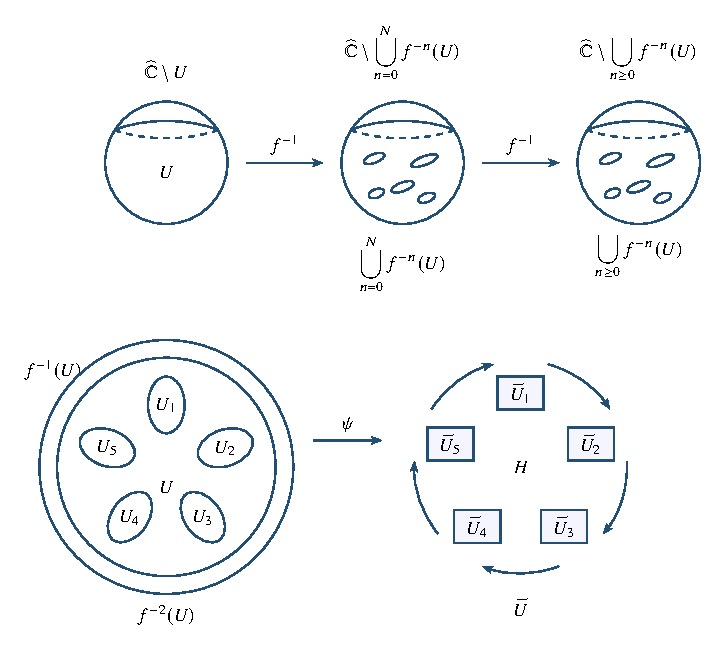
\includegraphics[width=.91\textwidth]{cd12-fig-01.pdf}
\FigureTag{CD12.1}{fig:cd12-01}
\end{figure}
\setcounter{theorem}{49}\begin{theorem}[Principle 2: pointwise surgery]
Let \(f:\widehat{\mathbb C}\to\widehat{\mathbb C}\) be quasiregular and \(X\subset\widehat{\mathbb C}\) open. Suppose
\(\partial_{\bar z}f=0\) almost everywhere on \(\widehat{\mathbb C}\setminus X\), \(f\) is \(K\)-quasiconformal on \(X\), and there is \(N\ge1\) such that
\[
\max_{z\in X}\#\bigl(\operatorname{orbit}(z)\cap X\bigr)\le N.
\]
Then \(f\) is quasirational.
\end{theorem}
% Source page 5

% Source page 6
% BLOG-CONTENT-END
\end{document}
